\documentclass{beamer}
\usepackage[utf8]{inputenc}
\usepackage[spanish]{babel}
\usetheme{Goettingen}
\usecolortheme{default}
\useoutertheme{shadow}
\useinnertheme{rectangles}
\graphicspath{ {./figures/} }
\title[UNAM]{Hola Mundo con JEE y Netbeans}
\subtitle{Ingeniería de software}
\author[Miguel]{Miguel Angel Piña Avelino}
\institute[UNAM]{
  Facultad de Ciencias, UNAM
}
\date{\today}

\begin{document}

\frame{\titlepage}

\begin{frame}
  \frametitle{Índice}
  \tableofcontents
\end{frame}

\section{Introducción}
\begin{frame}
  \frametitle{Introducción}
  Vamos a comenzar a conocer sobre JEE y netbeans a través del desarrollo de un
  primer ``Hola Mundo''.
\end{frame}

\section{Objectivo}

\begin{frame}
  \frametitle{Objectivo}
  \begin{itemize}
    \item Concer más sobre netbeans
    \item Conocer más sobre JEE
    \item Desarrollar nuestro primer ``hola mundo''
    \item Introducción a los conceptos de JEE
  \end{itemize}
\end{frame}

\begin{frame}
  \frametitle{Configuraciones previas}
  Vamos a verificar que Netbeans pueda soportar el desarrollo de aplicaciones
  web con Java.\\
  Para hacer esto, es necesario verificar que al momento de crear un proyecto
  tengan algo similar a la imagen
  \begin{figure}[ht]
    \centering
    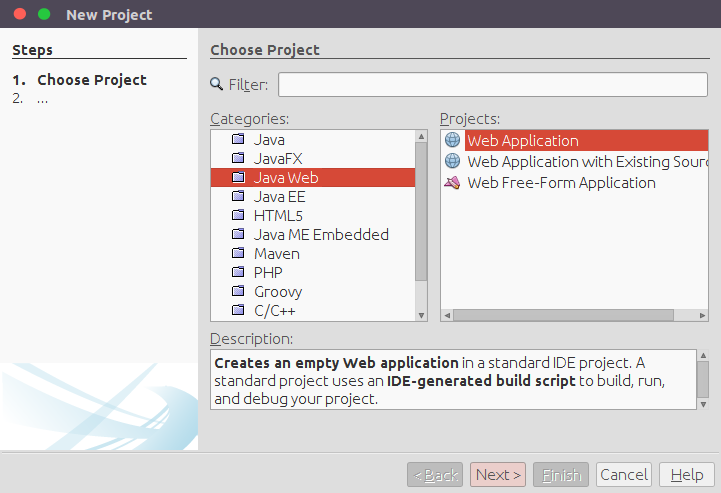
\includegraphics[scale=0.25]{figures/proyecto.png}
    \caption{\label{fig:Proyecto} Declaración del proyecto }
  \end{figure}

\end{frame}

\begin{frame}
  \frametitle{Creación del proyecto}
  Ahora vamos a crear nuestro proyecto en Netbeans, por lo que debemos hacer
  algo similar a lo de la imagen.
  \begin{figure}[ht]
    \centering
    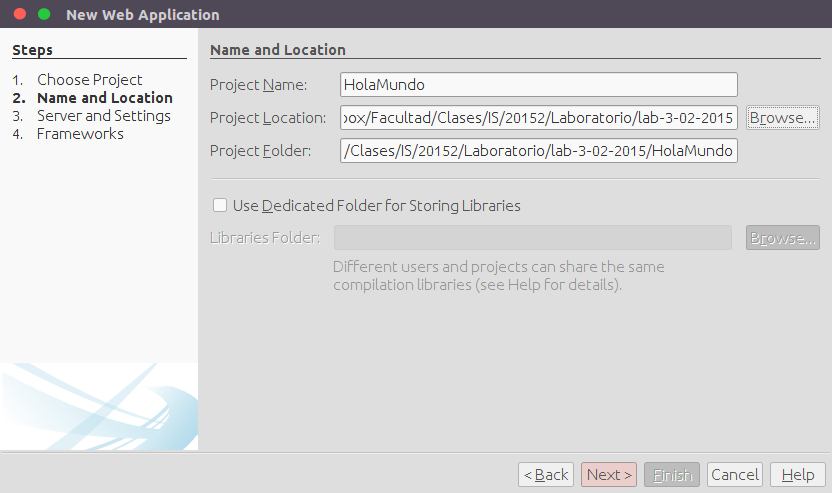
\includegraphics[scale=0.25]{figures/holamundo.png}
    \caption{\label{fig:HolaMundo} Nombre del proyecto}
  \end{figure}

\end{frame}


\begin{frame}
  \frametitle{Selección del servidor}
  Seleccionamos el servidor, el que vamos a usar es el de glassfish.
  \begin{figure}[ht]
    \centering
    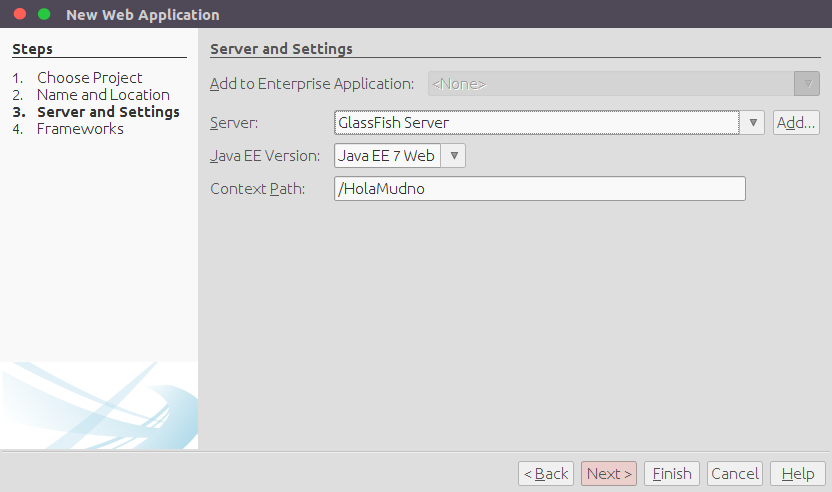
\includegraphics[scale=0.25]{figures/serversettings.png}
    \caption{\label{fig:serversettings} Selección del servidor}
  \end{figure}

\end{frame}

\begin{frame}
  \frametitle{Selección de frameworks}
  Por el momento, no debemos de seleccionar ninguno.
  \begin{figure}[ht]
    \centering
    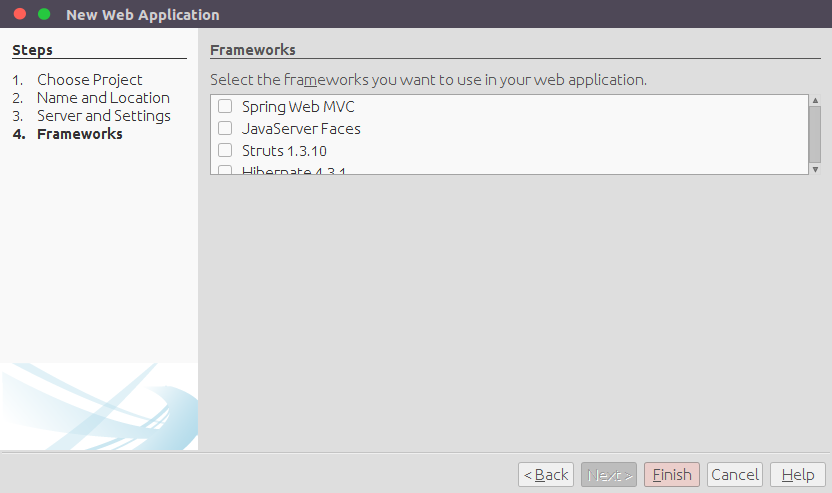
\includegraphics[scale=0.25]{figures/frameworks.png}
    \caption{\label{fig:frameworks} Framework}
  \end{figure}

\end{frame}
\begin{frame}
  \frametitle{Proyecto creado}
  Con esto hemos creado nuestro primer proyecto en netbeans.

  \begin{figure}[ht]
    \centering
    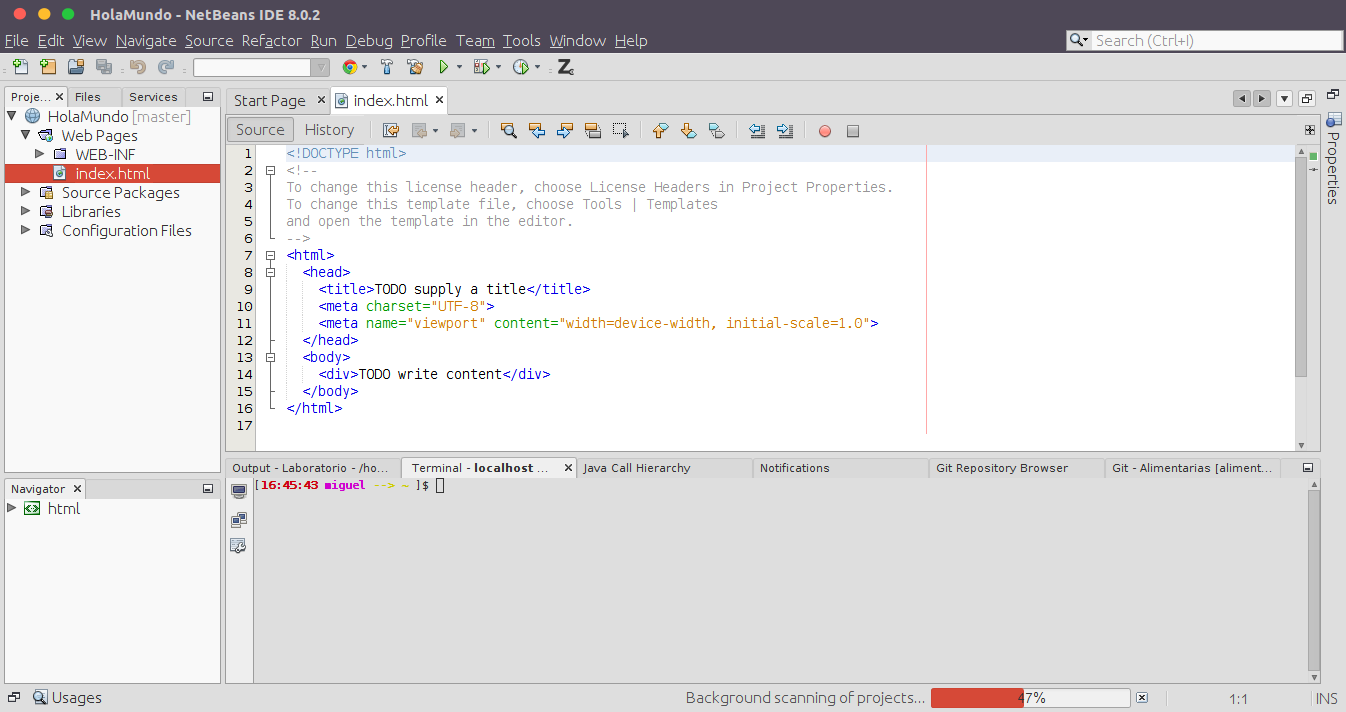
\includegraphics[scale=0.20]{figures/Index.png}
    \caption{\label{fig:Proyecto} Primer proyecto}
  \end{figure}

\end{frame}
\end{document}

%%% Local Variables:
%%% mode: latex
%%% TeX-master: t
%%% End:
